\documentclass[border=4pt]{standalone}
\usepackage{fontspec}
\usepackage{amsmath}
\usepackage{unicode-math}
\setmainfont{Latin Modern Roman}
\setmathfont{Latin Modern Math}
\usepackage{pgfplots}
\usepackage{pgfplotstable}
\pgfplotsset{compat=1.18}
\usepackage{tkz-euclide}
\usetikzlibrary{arrows.meta,calc,angles,quotes,patterns,3d,backgrounds}
\definecolor{ink}{HTML}{123428}
\definecolor{asy}{HTML}{475569}
\definecolor{mint}{HTML}{86e0bd}
\tikzset{asym/.style={asy, line width=0.9pt, dash pattern=on 5pt off 3.5pt},
         guide/.style={gray!70, line width=0.6pt, densely dotted},
         dot/.style={circle, inner sep=0pt, minimum size=5pt, draw=white, line width=0.5pt},
         odot/.style={circle, inner sep=0pt, minimum size=5.5pt, fill=white, line width=1pt},
         lab/.style={font=\footnotesize, inner sep=1.5pt, text=ink}}
\begin{document}
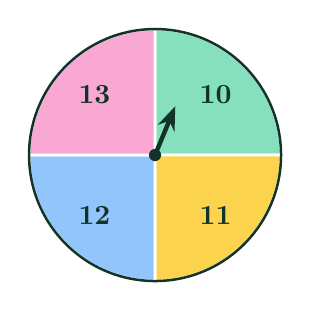
\begin{tikzpicture}
\fill[fill={rgb,255:red,134;green,224;blue,189}, draw=white, line width=1pt] (0,0) -- (90.000:1.6) arc[start angle=90.000, end angle=0.000, radius=1.6cm] -- cycle;
\node[font=\bfseries, text=ink] at (45.000:1.088) {10};
\fill[fill={rgb,255:red,252;green,211;blue,77}, draw=white, line width=1pt] (0,0) -- (0.000:1.6) arc[start angle=0.000, end angle=-90.000, radius=1.6cm] -- cycle;
\node[font=\bfseries, text=ink] at (-45.000:1.088) {11};
\fill[fill={rgb,255:red,147;green,197;blue,253}, draw=white, line width=1pt] (0,0) -- (-90.000:1.6) arc[start angle=-90.000, end angle=-180.000, radius=1.6cm] -- cycle;
\node[font=\bfseries, text=ink] at (-135.000:1.088) {12};
\fill[fill={rgb,255:red,249;green,168;blue,212}, draw=white, line width=1pt] (0,0) -- (-180.000:1.6) arc[start angle=-180.000, end angle=-270.000, radius=1.6cm] -- cycle;
\node[font=\bfseries, text=ink] at (-225.000:1.088) {13};
\draw[ink, line width=0.9pt] (0,0) circle (1.6);
\draw[ink, line width=1.6pt, -{Stealth[length=3mm]}] (0,0) -- (67.500:0.672);
\fill[ink] (0,0) circle (2.2pt);
\end{tikzpicture}
\end{document}
